\documentclass[11pt]{article}

\usepackage[T1]{fontenc}
\usepackage[utf8]{inputenc}
\usepackage{microtype}
\usepackage[a4paper,margin=28mm]{geometry}
\usepackage{amsmath,amssymb,amsthm,mathtools}
\usepackage{booktabs,array,tabularx,longtable}
\usepackage{enumitem}
\usepackage{tikz}
\usetikzlibrary{arrows.meta,fit,positioning}
\usepackage{pgfplots}
\pgfplotsset{compat=1.18}
\usepackage{xcolor}
\usepackage{hyperref}
\usepackage[nameinlink,capitalise,noabbrev]{cleveref}
\usepackage{listings}
\usepackage{url}
% Author information for the manuscript and arXiv submission.
\newcommand{\PaperAuthor}{Vladislav Kuznetsov}
\newcommand{\PaperAffiliation}{Moscow Institute of Physics and Technology (MIPT), Dolgoprudny, Russia}


\hypersetup{
  colorlinks=true,
  linkcolor=blue!55!black,
  citecolor=blue!55!black,
  urlcolor=blue!55!black,
  pdftitle={Exhaustive Boundary-Layer Certification for Megaminx via Neural-Guided Beam Cascades},
  pdfauthor={\PaperAuthor}
}
\setlist{nosep}
\lstset{basicstyle=\ttfamily\small,breaklines=true,columns=fullflexible}

\newtheorem{theorem}{Theorem}
\newtheorem{lemma}[theorem]{Lemma}
\newtheorem{proposition}[theorem]{Proposition}
\newtheorem{corollary}[theorem]{Corollary}
\theoremstyle{definition}
\newtheorem{definition}[theorem]{Definition}
\newtheorem{remark}[theorem]{Remark}

\newcommand{\FTM}{\mathrm{FTM}}
\newcommand{\Rsolve}{\mathcal{R}}
\newcommand{\Gpair}[2]{\Rsolve_{\Omega}(G_{#1},G_{#2})}

\title{Exhaustive Boundary-Layer Certification for Megaminx\\
  via Neural-Guided Beam Cascades}
\author{\PaperAuthor\\\small \PaperAffiliation}
\date{July 2026}

\begin{document}
\maketitle

\begin{abstract}
We certify one-move reductions for two adjacent phase pairs in a subgroup-chain
Megaminx solver under the face-turn metric.  The separate worst-case solving
distances of phases 3 and 4 are 14 and 8, while those of phases 5 and 6 are 13
and 13.  A boundary-layer argument shows that improving either sum by one
requires checking only compositions for which both constituent coordinates
are maximally distant from their target subgroups.  This reduces combined
quotients of sizes $14{,}234{,}011{,}545{,}600$ and
$1{,}664{,}617{,}163{,}489{,}280$ to exhaustive frontiers of $536{,}572$ and
$407{,}628$ physical states.  Exact local rewrites certify $8{,}664$ states.
For the remaining $935{,}536$, compact neural action-ranking models guide
batched beam-search cascades that produce bounded solution words.  The models
and search scores are not proof objects.  A deterministic checker requires
exact frontier coverage, while separately implemented replay engines validate
every word proposed by neural-guided search; exact-rewrite words are also
replayed physically.  In the published run the models supplied $935{,}536$
direct certificates in approximately $6.25$ active A100 GPU-hours, excluding
training, preprocessing, and verification.  We thereby obtain the ambient-FTM
bounds
\[
  \Gpair{5}{7}\le 21,
  \qquad
  \Gpair{7}{9}\le 25.
\]
Relative to the externally reported 114-move phase chain, these local results
give the conditional bound 112; together with the separately certified
color-neutral first-phase result, they give the likewise conditional bound
111.  The paper is accompanied by the complete certificate databases, pinned
phase-table reconstruction, and fail-closed verification software.
\end{abstract}

\section{Introduction}
\label{sec:introduction}

The Megaminx is a face-turning permutation puzzle with $12$ pentagonal faces,
$20$ movable corners, and $30$ movable edges.  Its state space is too large for
a direct breadth-first computation of the maximum solution length.  As in the
largest certified computations for the Rubik's Cube, useful upper bounds are
therefore obtained by decomposing the solve along a subgroup chain and
certifying the worst-case cost of each transition
\cite{korf1997,kunkle2007,rokicki2013}.

The phase chain studied here was developed in the public Megaminx solver of
Botz~\cite{botz2026dataset}.  In the face-turn metric, its separately computed
phase bounds include the consecutive pairs
\[
  14+8=22
  \qquad\text{and}\qquad
  13+13=26.
\]
The complete externally reported chain has length $114$.  This paper does not
reconstruct the computations outside the two phase pairs considered below;
consequences for that global value are therefore stated conditionally.

Our starting point is a simple boundary-layer observation.  To lower a sum $a+b$
of two integer-valued phase bounds to $a+b-1$, every state for which at least
one constituent phase has distance below its maximum is already harmless.
Only states whose two coordinates are simultaneously maximal require new
solutions.  For phases 3 and 4 this boundary consists of physical lifts of the
Cartesian product
of $212$ and $2{,}531$ coordinates; for phases 5 and 6 it is a product of
$3{,}484$ and $117$ coordinates.  Thus two combined quotients containing
roughly $1.42\times10^{13}$ and $1.66\times10^{15}$ coordinates reduce to
$536{,}572$ and $407{,}628$ explicit proof obligations.

Closing nearly one million individually specified obligations remains a
substantial search problem.  We train compact neural models directly on the
two combined quotients using sparse supervision from random trajectories.
The models rank actions inside one beam per root, evaluated in batches across
many roots on a GPU.  A staged schedule applies narrow beams to the
full unresolved set and reserves wider beams for the diminishing survivor
tail.  Exact local rewriting closes $8{,}664$ states, and the neural-guided
search produces bounded words for the remaining $935{,}536$ in approximately
$6.25$ active A100 GPU-hours.  This aggregate excludes model training, phase
tables, exact rewriting, process gaps, and final replay.

The neural computation is deliberately outside the trusted proof base.  A
checkpoint need not estimate a true distance, and an individual beam search
need not be complete.  The proof uses only the resulting words: the checker
requires an exact partition of the exhaustive frontier, binds every record to
its physical state, enforces the pair-specific length limit, and replays every
direct word without loading a model.  This yields the certified ambient-FTM
upper bounds
\[
  \Gpair{5}{7}\le21,
  \qquad
  \Gpair{7}{9}\le25.
\]

The contributions are therefore:
\begin{enumerate}
  \item a general boundary-layer reduction for improving two consecutive
    subgroup phases by one move;
  \item complete physical constructions of the two simultaneous-maximal
    frontiers, including exact lifting and coordinate round trips;
  \item a proof-oriented neural beam cascade that generates independently
    checkable words for a fixed exhaustive worst-case frontier rather
    than a sampled test distribution; and
  \item deterministic certificate checks establishing the two local
    bounds and, conditional on the reported surrounding phase chain, the
    global reductions $114\to112$ and $114\to111$ when combined with the
    separate color-neutral first-phase result.
\end{enumerate}

We do not claim a new generic beam-search algorithm, exact combined distances,
or ordinary graph diameters.  In particular, combined paths are allowed to
leave their source subgroups under the full FTM move alphabet.  The
mathematical result is exhaustive coverage by bounded words; the learned
search is an effective way of discovering those words.

\begin{figure}[t]
\centering
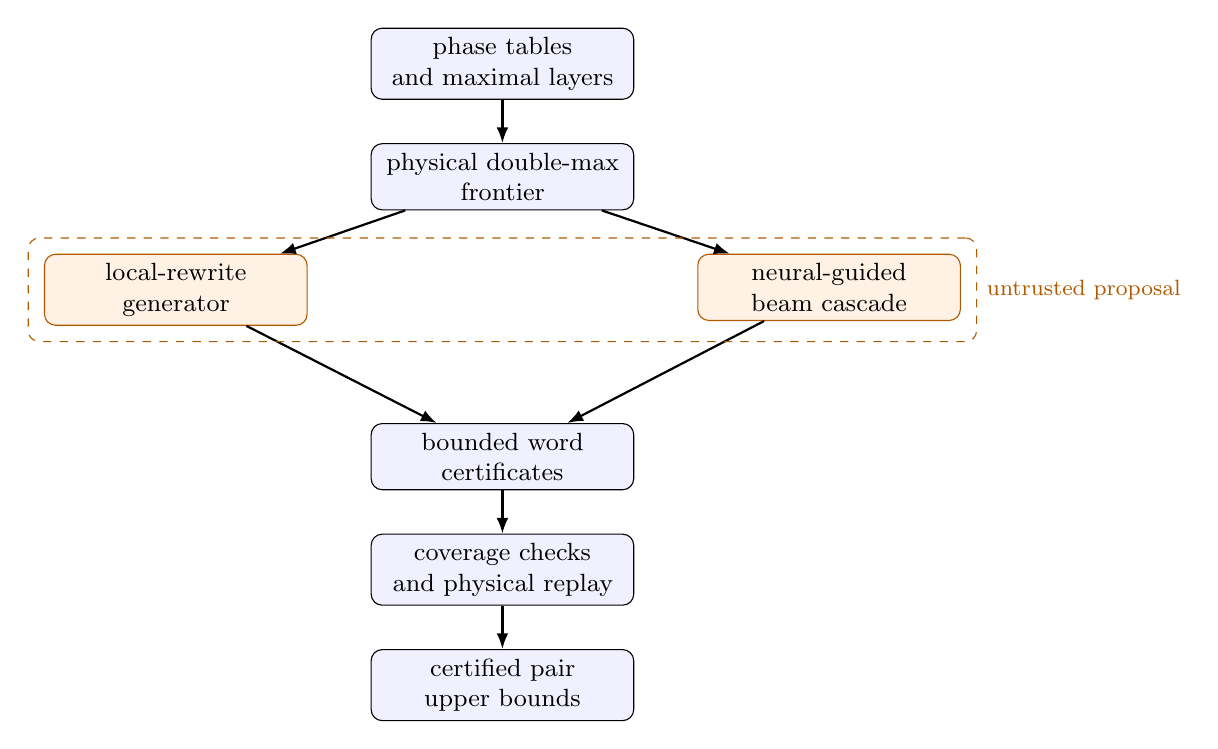
\begin{tikzpicture}[
  node distance=5.5mm and 8mm,
  box/.style={draw,rounded corners,align=center,minimum height=8mm,
              text width=31mm,font=\small},
  checked/.style={box,fill=blue!6},
  proposer/.style={box,fill=orange!10,draw=orange!70!black},
  arrow/.style={-{Latex[length=2mm]},thick}
]
  \node[checked] (tables) {phase tables\\and maximal layers};
  \node[checked,below=of tables] (frontier) {physical double-max\\frontier};
  \node[proposer,below left=of frontier] (rewrite) {local-rewrite\\generator};
  \node[proposer,below right=of frontier] (neural) {neural-guided\\beam cascade};
  \node[checked,below=27mm of frontier] (certs) {bounded word\\certificates};
  \node[checked,below=of certs] (replay) {coverage checks\\and physical replay};
  \node[checked,below=of replay] (bounds) {certified pair\\upper bounds};
  \draw[arrow] (tables)--(frontier);
  \draw[arrow] (frontier)--(rewrite);
  \draw[arrow] (frontier)--(neural);
  \draw[arrow] (rewrite)--(certs);
  \draw[arrow] (neural)--(certs);
  \draw[arrow] (certs)--(replay);
  \draw[arrow] (replay)--(bounds);
  \node[draw=orange!70!black,dashed,rounded corners,fit=(rewrite)(neural),
        inner sep=2mm,
        label={[font=\footnotesize,text=orange!70!black]right:untrusted proposal}] {};
\end{tikzpicture}
\caption{Proof pipeline and trust boundary.  Both search procedures propose
words; neither procedure is trusted.  The proof consumes only the exhaustive
frontier, the stored words, and the results of deterministic coverage and
replay checks.}
\label{fig:proof-pipeline}
\end{figure}

\section{Related work}
\label{sec:related-work}

\paragraph{Certified bounds for permutation puzzles.}
Group actions, Cayley graphs, and subgroup methods provide the standard
language for permutation puzzles~\cite{joyner2008}.  Pattern databases and
memory-efficient heuristic search made large puzzle spaces computationally
accessible~\cite{korf1997,culberson1998}.  Kunkle and Cooperman used
computational group methods to establish a 26-move upper bound for the Rubik's
Cube~\cite{kunkle2007}; Rokicki, Kociemba, Davidson, and Dethridge later
certified that the diameter in the half-turn metric is 20~\cite{rokicki2013}.
These works exemplify the separation between a large discovery computation
and a smaller, auditable verification argument.  The present computation uses
the same high-level discipline, but its finite obligation is a pair of
maximal-layer products in a Megaminx subgroup chain.

\paragraph{Learned heuristic search.}
DeepCubeA combines a learned cost-to-go function with batched heuristic search
and solves random instances of several puzzles, including the Rubik's
Cube~\cite{agostinelli2019}.  EfficientCube demonstrates that comparatively
simple self-supervision from goal-rooted scrambles can support neural-guided
beam search~\cite{takano2023}.  More recent work uses neural distance models
and massively parallel beam search on larger Rubik's Cubes
\cite{chervov2025}.  Our training signal and model architecture are secondary
to the certificate result: the models need only rank sufficiently many promising actions
to find a valid word for every member of a fixed exhaustive frontier.

\paragraph{Beam portfolios and batched learned heuristics.}
Restarting a learned beam search with progressively larger widths has appeared
in combinatorial optimization~\cite{cohenbeck2021}.  GPU batching of expensive
learned heuristics is likewise established in heuristic-search research
\cite{greco2022,futuhisturtevant2026}.  Accordingly, we describe our procedure
as a \emph{beam cascade} or staged search portfolio, not as a new beam-search
algorithm.  Its role in our computation is proof-oriented budget allocation: each
stage searches only unresolved members of an already exhaustive family, and
each success is persisted as a model-independent certificate.

\paragraph{Megaminx computations.}
The coordinates, phase numbering, move conventions, and reported global bound
used here originate in the software and accompanying analysis of
Botz~\cite{botz2026dataset,botzsource}.  The public history begins with the
116-move chain~\cite{botz2025bound116}.  A later table correction confirmed,
rather than improved, that value~\cite{botz2025correction}; two subsequent
reports reduced the last-phase contribution $26\to25\to24$, giving
$116\to115\to114$~\cite{rokicki2025bound115,rokicki2025bound114,botz2026bound114}.
These are external software and forum reports, not computations regenerated in
this paper.  The separate phase-1 result proves that allowing
the first block target to vary over all $20$ corners lowers its worst-case cost
from 10 to 9~\cite{kuznetsov2026phase1}.  Neither that result nor the present
paper reruns all external computations behind the reported 114-move chain;
the local theorems are unconditional, whereas the global arithmetic is not.

\section{Metric, coordinates, and boundary layers}
\label{sec:mathematics}

\subsection{Face-turn metric and subgroup coordinates}
\label{sec:metric-coordinates}

Let a face symbol denote a clockwise turn through one fifth of a revolution.
For a set $F$ of faces, write
\[
  \Sigma_F=\{X^k:X\in F,\ 1\leq k\leq4\}.
\]
Every element of $\Sigma_F$ has cost one.  Thus $X$, $X^2$, $X^3$, and
$X^4=X^{-1}$ are each one move in the face-turn metric (FTM); rotations,
slice turns, and identity moves are not in the alphabet.  In particular,
$\Sigma_F$ is symmetric.  If $w=s_1\cdots s_m$ is a word, then
$|w|=m$, and its tokens act from left to right:
\[
  x\mathbin{\cdot}w
  =(((x\mathbin{\cdot}s_1)\mathbin{\cdot}s_2)\cdots)
    \mathbin{\cdot}s_m.
\]
This convention matters for the physical lifting below.

Let $\Omega$ denote the full $48$-move FTM alphabet obtained by taking all
four nonidentity powers of all $12$ faces.  Words over $\Omega$ may temporarily
leave a subgroup; only their start and target memberships matter for an
ambient FTM bound.

The part of the subgroup chain used in this work is
\begin{align*}
  G_5&=\langle U,R,F,L,\mathrm{BR},\mathrm{BL},\mathrm{FR}\rangle,
  &G_6&=\langle U,R,F,L,\mathrm{BR},\mathrm{BL}\rangle,\\
  G_7&=\langle U,R,F,L,\mathrm{BR}\rangle,
  &G_8&=\langle U,R,F,L\rangle,\\
  G_9&=\langle U,R,F\rangle.
\end{align*}
For $G_i$ we use the FTM alphabet containing the four nonidentity powers of
each displayed generator of $G_i$; denote it by $\Sigma_i$.  Hence
$\Sigma_{i+1}\subseteq\Sigma_i$ for the transitions considered here.

\begin{definition}[Target-solving distance]
\label{def:target-distance}
Let $A\geq B$ be two groups in the chain, and let $\Gamma$ be a symmetric FTM
alphabet.  For a state $x\in A$, define
\[
  d_{\Gamma}(x,B)
    =\min\bigl\{|w|:w\in\Gamma^*,\ x\mathbin{\cdot}w\in B\bigr\},
\]
and define the worst-case target-solving radius over starts in $A$ by
\[
  \Rsolve_{\Gamma}(A,B)=\max_{x\in A}d_{\Gamma}(x,B).
\]
For a phase table we use $\Gamma=\Sigma_A$ and abbreviate
\begin{align*}
  \rho(A,B)&=\Rsolve_{\Sigma_A}(A,B),\\
  d_{A,B}(Bx)&=d_{\Sigma_A}(x,B),\\
  \mathcal M(A,B)
    &=\{Bx\in B\backslash A:d_{A,B}(Bx)=\rho(A,B)\}.
\end{align*}
\end{definition}

The distance is independent of the representative of a left $B$-coset: if
$x'=bx$ with $b\in B$, then $x'\mathbin{\cdot}w\in B$ if and only if
$x\mathbin{\cdot}w\in B$.  When $\Gamma=\Sigma_A$, $\rho(A,B)$ is the
eccentricity of the target vertex $B$ in the Schreier graph on
$B\backslash A$ generated by $\Sigma_A$.  It is not, by definition, the
ordinary graph diameter, which maximizes distance over arbitrary pairs of
vertices.  We therefore use ``target-solving radius'' rather than
``diameter'' for the quantities proved by the phase tables.  The combined
claims below allow $\Gamma=\Sigma_5$, which may be larger than the source
alphabet, and also state the resulting ambient $\Gamma=\Omega$ bounds.  Their
solution paths need not remain inside the source subgroup and hence should not
be described as diameters of those phase Schreier graphs.

\subsection{A complete physical lift of two coordinates}
\label{sec:physical-lift}

Let $A\geq B\geq C$.  For each $p\in B\backslash A$, fix an optimal lowering
word $u_p\in\Sigma_A^*$ such that
\[
  p\mathbin{\cdot}u_p=B,
  \qquad |u_p|=d_{A,B}(p).
\]
The first equality implies $p=B u_p^{-1}$.  For each
$q\in C\backslash B$, fix a physical representative $r_q\in B$ with
$Cr_q=q$.  Define the lifted state
\begin{equation}
  \lambda(p,q)=r_q\mathbin{\cdot}u_p^{-1}.
  \label{eq:physical-lift}
\end{equation}
Thus, under left-to-right replay, the product order is the representative of
the \emph{second} coordinate followed by the inverse of the lowering word for
the \emph{first} coordinate.

\begin{lemma}[Lifting and product order]
\label{lem:maximal-lifting}
For every $(p,q)\in(B\backslash A)\times(C\backslash B)$, the state
$\lambda(p,q)$ satisfies
\begin{align}
  B\lambda(p,q)&=p,
  \label{eq:lift-first-coordinate}\\
  \lambda(p,q)\mathbin{\cdot}u_p&=r_q,
  \label{eq:lift-intermediate}\\
  C\bigl(\lambda(p,q)\mathbin{\cdot}u_p\bigr)&=q.
  \label{eq:lift-second-coordinate}
\end{align}
Moreover, the lift is complete in the following sense.  Given any $x\in A$,
put $p=Bx$ and $q=C(x\mathbin{\cdot}u_p)$.  Then
\begin{equation}
  Cx=C\lambda(p,q).
  \label{eq:lift-completeness}
\end{equation}
Consequently, one lifted state for each pair $(p,q)$ covers every combined
$C$-coset that can arise after the chosen optimal first-phase lowering word.
Injectivity is neither assumed nor required.
\end{lemma}

\begin{proof}
Because $r_q\in B$ and $p=B u_p^{-1}$,
\[
  B\lambda(p,q)=B r_q u_p^{-1}=B u_p^{-1}=p.
\]
Applying $u_p$ cancels its inverse in~\eqref{eq:physical-lift}, giving
$r_q$ and hence the second coordinate $Cr_q=q$.

For completeness, $p=Bx$ and $p\mathbin{\cdot}u_p=B$ imply that
$y=x\mathbin{\cdot}u_p$ belongs to $B$.  If $q=Cy$, then $y$ and $r_q$
are in the same left $C$-coset, so $y=cr_q$ for some $c\in C$.  Therefore
\[
  x=y\mathbin{\cdot}u_p^{-1}
    =c r_q\mathbin{\cdot}u_p^{-1}
    =c\lambda(p,q),
\]
which proves~\eqref{eq:lift-completeness}.
\end{proof}

The artifact materializes~\eqref{eq:physical-lift} in a full physical
Megaminx state rather than combining coordinate integers.  It then checks
\cref{eq:lift-first-coordinate,eq:lift-intermediate,eq:lift-second-coordinate}
for every raw pair.  Although the proof does not need injectivity, the two
concrete lifted products in this work happen to contain no duplicate physical
states.

\subsection{Boundary-layer reduction}
\label{sec:boundary-layer-reduction}

\begin{lemma}[Boundary-layer reduction]
\label{lem:boundary-layer}
Let $A\geq B\geq C$ be finite groups with symmetric generating alphabets
$\Sigma_B\subseteq\Sigma_A$.  Let $\Gamma$ be any symmetric FTM alphabet
containing $\Sigma_A$, and put
\[
  a=\rho(A,B),
  \qquad b=\rho(B,C).
\]
Construct $\lambda(p,q)$ as in~\cref{lem:maximal-lifting}.  Suppose that
for every
\[
  (p,q)\in\mathcal M(A,B)\times\mathcal M(B,C)
\]
there is a word over $\Gamma$ of length at most $a+b-1$ that takes
$\lambda(p,q)$ into $C$.  Then
\[
  \Rsolve_{\Gamma}(A,C)\leq a+b-1.
\]
\end{lemma}

\begin{proof}
Fix $x\in A$ and set $p=Bx$.  If $d_{A,B}(p)\leq a-1$, first apply the
optimal word $u_p$ and then solve the resulting element of $B$ into $C$ in at
most $b$ moves.  The total is at most $a+b-1$.

It remains to consider $p\in\mathcal M(A,B)$, so $|u_p|=a$.  Put
$y=x\mathbin{\cdot}u_p\in B$ and $q=Cy$.  If
$d_{B,C}(q)\leq b-1$, the same sequential argument costs at most
$a+b-1$.  Otherwise $q\in\mathcal M(B,C)$.  By
\cref{lem:maximal-lifting}, $Cx=C\lambda(p,q)$.  Ambient target-solving
distance to $C$ depends only on this left coset, and the assumed frontier word
therefore solves $x$ in at most $a+b-1$ moves.  These cases exhaust $A$.
\end{proof}

The lemma isolates precisely the simultaneous-maximal boundary.  It does not
claim that a search over this boundary is complete: completeness comes from
enumerating the entire product and replaying a valid bounded word for each
member.

\subsection{Exact phase data and exhaustive frontiers}
\label{sec:phase-data}

The proof treats the implementation coordinates as group quotients only after
an exact coordinate-contract audit.  For each phase, the coordinate is the
orbit of a tuple of labelled, oriented pieces under the source generators.
The builder checks that every target generator fixes the target tuple, that
the coordinate ranks and transitions are well defined, and that the BFS
reaches the full declared coordinate set.  A Schreier--Sims audit on the
pinned $120$-position actions recomputes
\begin{align*}
 [G_5:G_7]&=208{,}099{,}584\cdot68{,}400,\\
 [G_7:G_9]&=64{,}157{,}184\cdot25{,}945{,}920,
\end{align*}
as well as the two intermediate subgroup orders.  To see why these checks
suffice, let $n_1,n_2$ be the two coordinate counts in either pair.  Target
invariance makes each coordinate orbit a quotient by a stabilizer containing
the stated target subgroup, so
\(n_1\leq[A:B]\) and \(n_2\leq[B:C]\).  The exact order audit gives
\(n_1n_2=[A:C]=[A:B][B:C]\); hence both inequalities are equalities and the
target stabilizers are exactly $B$ and $C$.  Thus the coordinate fibers are
the left cosets used in \cref{def:target-distance}, rather than merely hashes
that agree in sampled tests.

\begin{proposition}[Phase-table data]
\label{prop:phase-data}
Complete breadth-first phase tables, regenerated from the pinned move and
coordinate definitions, establish the following target-solving data.
\begin{center}
\begingroup
\small
\setlength{\tabcolsep}{3.5pt}
\begin{tabularx}{\textwidth}{@{}cc>{\raggedright\arraybackslash}Xrrrr@{}}
\toprule
Phase & Transition & Source faces & $|\Sigma_A|$ & $|B\backslash A|$
  & $\rho(A,B)$ & $|\mathcal M(A,B)|$ \\
\midrule
3 & $G_5\to G_6$ & $U,R,F,L,\mathrm{BR},\mathrm{BL},\mathrm{FR}$
  & 28 & $208{,}099{,}584$ & 14 & 212 \\
4 & $G_6\to G_7$ & $U,R,F,L,\mathrm{BR},\mathrm{BL}$
  & 24 & $68{,}400$ & 8 & $2{,}531$ \\
5 & $G_7\to G_8$ & $U,R,F,L,\mathrm{BR}$
  & 20 & $64{,}157{,}184$ & 13 & $3{,}484$ \\
6 & $G_8\to G_9$ & $U,R,F,L$
  & 16 & $25{,}945{,}920$ & 13 & 117 \\
\bottomrule
\end{tabularx}
\endgroup
\end{center}
Here the radii are distances from the target cosets, in the sense of
\cref{def:target-distance}; no ordinary Schreier-graph diameter is asserted.
\end{proposition}

For phases 3 and 4, the combined quotient has
\begin{equation}
  |G_7\backslash G_5|
    =208{,}099{,}584\cdot68{,}400
    =14{,}234{,}011{,}545{,}600,
  \label{eq:pair34-quotient-size}
\end{equation}
whereas the simultaneous-maximal product contains only
\begin{equation}
  212\cdot2{,}531=536{,}572
  \label{eq:pair34-frontier-size}
\end{equation}
raw lifts.  For phases 5 and 6, the corresponding values are
\begin{align}
  |G_9\backslash G_7|
    &=64{,}157{,}184\cdot25{,}945{,}920
      =1{,}664{,}617{,}163{,}489{,}280,
  \label{eq:pair56-quotient-size}\\
  3{,}484\cdot117&=407{,}628.
  \label{eq:pair56-frontier-size}
\end{align}
The complete physical lifting check found respectively $536{,}572$ and
$407{,}628$ valid, pairwise distinct full states (maximum multiplicity one).
The absence of duplicates makes the displayed products the exact numbers of
stored obligations; the logical coverage in~\cref{lem:maximal-lifting} would
remain valid even if duplicates had occurred.

\begin{proposition}[Exhaustive certificate coverage]
\label{prop:certificate-coverage}
The regenerated maximal-layer products admit the following exact partitions.
\begin{center}
\begin{tabular}{@{}lrrrr@{}}
\toprule
Pair & Raw lifts & Exact-rewrite words & Direct words & Missing \\
\midrule
$3+4$ & $536{,}572$ & 203 & $536{,}369$ & 0 \\
$5+6$ & $407{,}628$ & $8{,}461$ & $399{,}167$ & 0 \\
\bottomrule
\end{tabular}
\end{center}
Across the two pairs this is an exhaustive partition
\[
  944{,}200=8{,}664+935{,}536
\]
into exact-rewrite and direct-certificate obligations.
For pair $3+4$, every replayed word has length at most 21 and in fact uses the
restricted alphabet $\Sigma_5$.  For pair $5+6$, every replayed word has
length at most 25: the $8{,}461$ exact-rewrite witnesses are words over
$\Sigma_5$, while all $399{,}167$ direct words use the restricted alphabet
$\Sigma_7\subseteq\Sigma_5$.  For every ID, the checker reconstructs the
prescribed physical lift and requires membership in exactly one part of the
partition.  Exact-rewrite words are replayed in the full physical
representation all the way to the solved state.  Direct words are replayed
independently in the combined quotient and in the full physical
representation to the appropriate target subgroup.  Thus the proposition
depends on the words and their exhaustive ID coverage, not on the method that
discovered them.
\end{proposition}

\begin{remark}[Alphabet scope]
\label{rem:alphabet-scope}
The distinction between $\Sigma_7$ and $\Sigma_5$ is substantive.  The neural
database alone covers only the complement of the exact-rewrite set, so its
$\Sigma_7$ words do not establish a restricted-alphabet bound for every
frontier state.  Pair $5+6$ preprocessing uses the first seven faces, so the
complete partition establishes a $\Sigma_5$ bound, but not a $\Sigma_7$
bound.  The ambient conclusion follows because
$\Sigma_7\subseteq\Sigma_5\subseteq\Omega$.  Pair $3+4$ likewise has a
$\Sigma_5$ conclusion because both parts of its partition use that alphabet.
\end{remark}

\subsection{Certified upper bounds}
\label{sec:certified-bounds}

\begin{theorem}[Phases 3 and 4]
\label{thm:pair34}
The combined target-solving radii satisfy
\[
  \Rsolve_{\Sigma_5}(G_5,G_7)\leq21,
  \qquad
  \Rsolve_{\Omega}(G_5,G_7)\leq21.
\]
\end{theorem}

\begin{proof}
By~\cref{prop:phase-data}, the consecutive radii are 14 and 8.  The
simultaneous-maximal product is exhausted by
\cref{eq:pair34-frontier-size}, and every member has a word of length at most
$21=14+8-1$ by~\cref{prop:certificate-coverage}.  Apply
\cref{lem:boundary-layer} with $(A,B,C)=(G_5,G_6,G_7)$ and
$\Gamma=\Sigma_5$.  The ambient statement follows because
$\Sigma_5\subseteq\Omega$.
\end{proof}

\begin{theorem}[Phases 5 and 6]
\label{thm:pair56}
The combined target-solving radii satisfy
\[
  \Rsolve_{\Sigma_5}(G_7,G_9)\leq25,
  \qquad
  \Rsolve_{\Omega}(G_7,G_9)\leq25.
\]
\end{theorem}

\begin{proof}
The two consecutive radii are 13 and 13 by~\cref{prop:phase-data}.  The
product in~\cref{eq:pair56-frontier-size} is exhaustive, and
\cref{prop:certificate-coverage} supplies a word of length at most
$25=13+13-1$ for every member.  The claim follows from
\cref{lem:boundary-layer} with $(A,B,C)=(G_7,G_8,G_9)$ and
$\Gamma=\Sigma_5$.  The ambient statement follows because
$\Sigma_5\subseteq\Omega$.
\end{proof}

Theorems~\ref{thm:pair34} and~\ref{thm:pair56} are upper bounds only.  We do
not provide lower-bound witnesses at distances 21 or 25, and therefore do not
claim exact combined radii or ordinary graph diameters.

\begin{corollary}[Conditional 112-move bound]
\label{cor:conditional-112}
Assume that the externally reported 114-move Megaminx phase chain is a valid
FTM upper bound under the same move convention, subgroup chain, and phase
composition semantics used here, and that it contains the separate
contributions $14+8$ for phases 3 and 4 and $13+13$ for phases 5 and 6.  Then
every Megaminx state is solvable in at most 112 FTM moves.
\end{corollary}

\begin{proof}
Replacing $14+8=22$ by~\cref{thm:pair34}'s bound 21 saves one move, and
replacing $13+13=26$ by~\cref{thm:pair56}'s bound 25 saves a second.  All
other contributions in the assumed chain are unchanged, so its total becomes
$114-1-1=112$.
\end{proof}

\begin{corollary}[Conditional 111-move bound]
\label{cor:conditional-111}
Under the hypotheses of~\cref{cor:conditional-112}, assume additionally that
the separately certified color-neutral first-phase reduction is compatible
with the same 114-move chain and saves one further move.  Then every Megaminx
state is solvable in at most 111 FTM moves.
\end{corollary}

\begin{proof}
Apply the additional one-move saving to the conditional bound in
\cref{cor:conditional-112}.
\end{proof}

The two local theorems are certified by this artifact.  The corollaries are
deliberately conditional because this work neither regenerates the complete
external 114-move computation nor proves compatibility of every surrounding
phase transition.

\section{Exhaustive frontier construction}
\label{sec:frontier}

The phase tables store an exact lowering distance and one deterministic
lowering move for every reachable coordinate.  A maximal record additionally
contains a physical $108$-byte Megaminx state, a verified optimal lowering
word, and masks of all possible first and last moves on optimal paths.  The
table builder derives the maximal layers from the generated distances; the
published counts are comparison controls and are not used to manufacture or
truncate those layers.

For each pair, the first maximal record is combined with the second maximal
record using the lifting rule of \cref{lem:maximal-lifting}.  The checker then
verifies, for every raw pair, that
\begin{enumerate}
  \item its first coordinate is the requested phase-$i$ antipode;
  \item the stored optimal phase-$i$ word reaches the exact chosen
    phase-$(i+1)$ representative;
  \item that intermediate state has the requested second coordinate; and
  \item the stored second-phase word reaches the next subgroup.
\end{enumerate}
Coordinate integers are never treated as physical states.  The raw order is
first-layer major and second-layer minor, and an explicit raw-to-unique map is
constructed without assuming injectivity.  In the regenerated data all
$536{,}572$ and $407{,}628$ physical states are distinct.

\subsection{Exact preprocessing}
\label{sec:exact-preprocessing}

Before neural search, the concatenation of the two optimal lowering words is
processed by exact local transformations.  Consecutive moves on one face are
combined in the face-turn metric; commuting and cancellable moves are
normalized; and meet-in-the-middle dictionaries test windows straddling the
phase boundary.  Every hash match is confirmed by comparing the complete
physical state, and every resulting word is replayed from the corresponding
frontier state.

The published reductions search through $4+4$ boundary windows.  Both runs
use the first seven faces, namely the $28$ FTM moves in $\Sigma_5$; pair 5+6
may therefore leave its source subgroup $G_7$ during preprocessing.  They
close $203$ and $8{,}461$ states respectively.  An
exhaustive symmetry analysis separately reconstructs all $60$
orientation-preserving rotations and retains only maps preserving all nested
subgroups of the pair.  In both cases the admissible stabilizer is the
identity.  Inversion is also rejected: it exchanges the left- and right-coset
conventions, and the exhaustive frontier is not closed under it.  Consequently
no nontrivial orbit reduction is hidden in the coverage counts.

The remaining obligations are therefore the exact ordered ID sets shown in
\cref{tab:coverage-partition}.  The equality in each row is a checked
partition, not a statistical coverage estimate.

\begin{table}[t]
\centering
\caption{Exhaustive partition of the simultaneous-maximal frontiers.}
\label{tab:coverage-partition}
\begin{tabular}{@{}lrrr@{}}
\toprule
Pair & Raw frontier & Exact rewrites & Direct words\\
\midrule
3+4 & 536,572 & 203 & 536,369\\
5+6 & 407,628 & 8,461 & 399,167\\
\midrule
Total & 944,200 & 8,664 & 935,536\\
\bottomrule
\end{tabular}
\end{table}

\section{Neural-guided certificate generation}
\label{sec:neural-search}

The direct certificates were discovered by two separately trained models, one
for each combined quotient.  They share an architecture and training
procedure, but their state colorings, action sets, depth scales, parameters,
and checkpoints are distinct.  \Cref{tab:model-specifications} summarizes the
certificate-generation configurations.

\begin{table}[t]
\centering
\caption{Combined quotient and model specifications.}
\label{tab:model-specifications}
\small
\begin{tabular}{@{}lrr@{}}
\toprule
Property & Pair 3+4 & Pair 5+6\\
\midrule
Transition & $G_5\to G_7$ & $G_7\to G_9$\\
Combined quotient size & 14,234,011,545,600 & 1,664,617,163,489,280\\
State positions & 120 & 120\\
Position classes & 43 & 67\\
FTM actions & 28 & 20\\
Random-walk $K_{\max}$ & 22 & 26\\
Trainable parameters & 619,996 & 802,260\\
Certificate length limit & 21 & 25\\
\bottomrule
\end{tabular}
\end{table}

\subsection{Exact quotient encodings}

Each state is a coloring of the $120$ oriented sticker positions induced by
the target subgroup: positions movable inside the target are collapsed to one
class, while the remaining positions retain fixed classes.  The problem
builder uses Schreier--Sims to check both the subgroup index and equality
between the intended target subgroup and the pointwise stabilizer of the
retained classes~\cite{seress2003}.  A simultaneous conjugacy check aligns every generated
sticker action with the independent physical move convention.  Thus the model
sees the intended combined quotient rather than an accidental coarsening.
The committed problem manifests are the inputs to certificate replay; the
artifact recomputes their group orders and physical-action alignment without
loading a checkpoint.

The network first applies a position-specific class embedding.  Equivalently,
for coloring $x=(c_1,\ldots,c_{120})$ it computes
\(
 e(x)=b+\sum_{p=1}^{120}W_{p,c_p}
\)
without materializing the full position--class one-hot vector.  Batch
normalization and the SiLU activation map this $64$-dimensional representation
to width $256$.  Each of two residual blocks has the form
\[
 h\leftarrow\operatorname{SiLU}\!\left(
 h+\operatorname{BN}_2\!\left(L_2(
 \operatorname{Dropout}(\operatorname{SiLU}(\operatorname{BN}_1(L_1(h)))))
 \right)\right).
\]
Dropout was zero in both published runs.  A final linear layer emits one
real-valued score per legal action; lower scores are searched first.

\subsection{Sparse trajectory supervision}
\label{sec:sparse-supervision}

Training examples are generated online by nontrivial random walks starting at
the target coordinate.  Consecutive moves on the same face are excluded
because their product is either one FTM move or the identity; quotient
self-loops are also rejected.  For a randomly selected trajectory pivot $x_t$,
let $a^-$ be the inverse of the preceding action and $a^+$ the sampled next
action.  Only these two outputs are supervised:
\begin{equation}
  \mathcal{L}(x_t)
  =\frac12\left(Q_\theta(x_t,a^-)-(t-1)\right)^2
  +\frac12\left(Q_\theta(x_t,a^+)-(t+1)\right)^2.
  \label{eq:sparse-loss}
\end{equation}
The diagnostic pair accuracy is the fraction for which
$Q_\theta(x_t,a^-)<Q_\theta(x_t,a^+)$.  The trajectory index $t$ is not asserted
to equal the shortest distance of $x_t$.  Accordingly, $Q_\theta$ is best
understood as a learned action-ranking score trained from noisy trajectory
depths, not as an exact distance table or a certified Q-function.

\begin{table}[t]
\centering
\caption{Training configuration used for both models, except for the
pair-specific random-walk limit.}
\label{tab:training-configuration}
\small
\begin{tabular}{@{}ll@{\qquad}ll@{}}
\toprule
Optimizer & AdamW & Learning rate & $10^{-4}$\\
Weight decay & $0.003$ & Gradient clip & $1$\\
Batch size & $1{,}024$ & Steps per epoch & $256$\\
Walk range & $2\ldots K_{\max}$ & Validation size & $16{,}384$\\
Seed & $42$ & Inference/training type & bfloat16\\
\bottomrule
\end{tabular}
\end{table}

For every sample, the walk length is uniform on the displayed integer range
and the pivot is uniform among its internal vertices.  Eligible nontrivial
moves are sampled uniformly after the same-face exclusion.  The pair-3+4
certificate run used epochs 1024 and 1120 of one training run; pair 5+6 used
epochs 864 and 3744.  These checkpoint identities record the run that found
the certificates, not a claim that their epochs are generally optimal.

\subsection{One beam per root, evaluated in batches}
\label{sec:batched-beam}

At each depth, every root maintains its own beam, visited set, last-face
context, and paths; only neural inference is shared across roots.  Scores are
the current one-step values $Q_\theta(x,a)$, not cumulative path scores.  At a
beam of width $B$ with $A$ actions, the implementation first obtains the best
\[
  C=\min\{BA,\max(A,16B)\}
\]
parent--action pairs before CPU deduplication.  It initially scans
\(\min\{C,\max(A,2B)\}\) candidates and scans the rest only if duplicates
prevent the next beam from filling.  Same-face continuations are masked.  The
goal test occurs immediately after applying an action; self-loops and then
previously visited keys are discarded.  A key is the pair
\((\text{coloring},\text{last face})\), because those two copies of one
coloring have different legal continuations.  The first $B$ surviving keys in
score order form the next beam.

\begin{lstlisting}[caption={One root of the batched beam search.  Model calls
for all active roots are fused in the implementation.},label={lst:inner-beam}]
beam := {(root, last_face = none, word = empty)}
visited := {(root, none)}
for depth := 1 .. length_limit:
    P := legal (parent, action) pairs from beam
    rank P by one-step score Q(parent, action), ascending
    next := empty
    for pair in bounded top-candidate window P:
        child := apply(pair)
        if child is target: return pair.word
        key := (child, face(pair.action))
        if child is a self-loop or key in visited: continue
        add key to visited and pair to next
        if |next| = beam_width: break
    if next is empty: return failure
    beam := next
return failure
\end{lstlisting}

Exact floating-point ties inherit whatever ordering the PyTorch device
produces; the search does not require that order to be reproducible.  Any returned word is replayed
in the combined quotient and on the corresponding physical state before it can
enter the certificate database.

\begin{lstlisting}[caption={Survivor beam cascade used for certificate discovery.},
                   label={lst:cascade}]
U := ordered set of unresolved frontier IDs
for (checkpoint, beam_width) in schedule:
    for bounded chunk C of U:
        words := batched_per_root_beams(C, checkpoint,
                                       beam_width, length_limit)
        for (id, word) in words:
            if replay_quotient(id, word) and replay_physical(id, word):
                persist_certificate(id, word, provenance)
    U := U minus all persisted certificate IDs
    stop if U is empty
require U is empty
\end{lstlisting}

The database is resumable: existing IDs are skipped, records are tied to
checksums of the physical state and proof problem, and a later stage may replace
a record only with a shorter word or the same length at a smaller beam width.
The production runner uses outer chunks of $10{,}000$ frontier IDs and root
minibatches that decrease from 128 at narrow widths to 16 at width 4096.  The
older pair-5+6 width-64 pass used an earlier low-batch implementation, which is
why its throughput is not compared directly with later tiers.  Beam width,
checkpoint identity, and batching record discovery provenance only.

\subsection{Published cascade schedules}

The survivor plot in \cref{fig:survivor-curves} shows the schedules; full
counts, timings, and checkpoint splits appear in \cref{app:cascade}.  Roughly
60\% of each direct-certificate set was found at its first beam tier, while
the maximum width was applied to only one pair-3+4 survivor and $28$
pair-5+6 survivors.  These observations do not isolate the causal effect of
beam width.  Pair 3+4 combines
epoch-1024 and epoch-1120 checkpoints at width 32; pair 5+6 switches from
epoch 864 at width 64 to epoch 3744 for subsequent tiers.  Moreover, every
later tier sees a survivor distribution selected by all earlier tiers.  We
therefore present the cascade as the successful certificate-generation
portfolio actually used, not as evidence that one beam width dominates
another.

\section{Certificate verification and trusted base}
\label{sec:verification}

The search computation answers an existential question for each frontier
state: it proposes a word that appears to reach the target subgroup within the
required limit.  Certification turns those proposals into a finite,
fail-closed proof.  In particular, neither a neural score nor a claim that a
beam exhausted its search space is accepted as evidence.

\subsection{Certificate records and exact coverage}

For each pair, the direct certificates are stored in a SQLite database.  A
row contains the raw state ID, a SHA-256 digest of its 108-byte physical state,
the byte-coded move word and its length, and discovery provenance consisting
of the beam width and checkpoint digest.  A second digest binds the ID, state,
word, and provenance fields.  Database metadata binds the complete collection
to the metric, target subgroup, proof length limit, combined-quotient
definition, physical composition file, and ordered list of unresolved IDs.

Let $I$ be the full raw frontier ID set, $E\subset I$ the IDs closed by exact
rewriting, and $N\subset I$ the IDs represented in the direct-certificate
database.  The checker constructs $I$ and $E$ from regenerated artifacts and
requires
\begin{equation}
  E\cap N=\varnothing,
  \qquad E\cup N=I.
  \label{eq:exact-partition}
\end{equation}
It rejects missing IDs, extra IDs, duplicates, malformed words, stale state
digests, metadata disagreement, and any word longer than the pair-specific
limit.  Thus a partial or interrupted search database cannot be mistaken for
a complete proof.

\subsection{Replay paths and the full-reproduction cross-check}

The proof checker replays every accepted direct word along the first two paths
below.  The full-reproduction entry points additionally require the third:
\begin{enumerate}
  \item the exact 120-position coloring of the combined quotient;
  \item an independently written Python implementation of the full edge and
    corner permutations and orientations; and
  \item a persistent Go verifier compiled against the pinned physical move
    definitions, receiving only the full-state bytes and canonical move word.
\end{enumerate}
The quotient replay establishes arrival at the intended combined target, and
the Python full-state replay applies the physical moves and tests membership in
$G_7$ or $G_9$.  In a full reproduction, the Go path repeats the physical
replay without parsing SQLite or importing the Python transition code.  Python
and Go then independently hash the canonical stream of ID, state bytes, and
word; the workflow requires equality of the SHA-256 transcript digest, first
and last IDs, record count, and maximum length.  Thus aggregate agreement
cannot hide a substituted or omitted record.  Exact-rewrite witnesses are
likewise replayed before their IDs enter $E$.

The committed historical reference reports record the complete Python replay
but predate the transcript-bound Go path and contain no Go transcript fields.
Accordingly, they are not evidence that this newer cross-check was executed for
the published snapshot; rather, the repository makes that cross-check a
fail-closed requirement of a fresh full reproduction.  The mathematical upper
bounds rely on exact coverage and deterministic word replay, while the Go path
is an additional implementation-diversity check on the physical action.

These checks address different failure modes.  Agreement between two
representations cannot by itself prove that the frontier is complete, while an
exact ID partition cannot show that a stored word has the advertised action.
The proof requires both \cref{eq:exact-partition} and successful replay.

\begin{table}[t]
\centering
\caption{Verification roles and their independence boundary.}
\label{tab:verification-roles}
\small
\renewcommand{\arraystretch}{1.12}
\begin{tabularx}{\textwidth}{@{}
  >{\raggedright\arraybackslash}p{0.22\textwidth}
  >{\raggedright\arraybackslash}p{0.25\textwidth}
  >{\raggedright\arraybackslash}X@{}}
\toprule
Component & Implementation & Property checked\\
\midrule
Frontier and partition & deterministic Python pipeline & complete
maximal-layer product and exact ID partition\\
Combined replay & pair-specific Python coloring & every direct word reaches
the intended combined target coordinate\\
Physical replay & Python \texttt{FullStateV1} & every direct word reaches the
physical target subgroup\\
Physical cross-check & persistent Go verifier & separately implemented replay
of the exact same transcript; it shares the pinned move convention\\
Exact rewrites & generated in Go, checked in Python & every accepted rewrite
word has the allowed alphabet and length and physically solves its state\\
\bottomrule
\end{tabularx}
\end{table}

The deterministic coverage checker is not presented as an independent second
implementation of the entire proof.  Independence here is narrower: the two
physical replay engines use separate code paths, and the transcript binding
ensures that they receive the same direct certificates.

\subsection{Regeneration checks}

The full workflow begins before certificate replay.  It downloads a pinned
upstream source archive after verifying its digest, builds the table generator
and verifiers, and regenerates the four complete phase tables.  For every
phase, the checker validates the reachable count, histogram, maximal distance,
maximal-layer count, predecessor structure, and all stored checksums.  It then
reconstructs every maximal physical representative and optimal lowering word,
forms the complete products from \cref{eq:pair34-frontier-size,eq:pair56-frontier-size},
checks the lifting identities of \cref{lem:maximal-lifting}, and regenerates
the exact-rewrite partition.

The published numerical controls are used only for comparison after
generation.  They are not loop bounds for truncating a table or manufacturing
a maximal layer.  Temporary outputs are written under distinct paths, and
payloads with missing records or inconsistent hashes cause the run to stop.

\subsection{Trusted and untrusted components}

The trusted computational base consists of the pinned move and coordinate
definitions, table construction, physical lifting, strict word parsers,
coverage logic, cryptographic hashes as integrity guards, and the replay
implementations.  The neural training code, checkpoints, floating-point
scores, batching order, beam widths, certificate timestamps, and GPU libraries
are outside that base.  The deterministic local-rewrite search is likewise a
word proposer: only its checked outputs enter the proof.  These components can
affect which word is found and how quickly, but cannot make an invalid or
absent word pass the checker.  This separation is the main reason learned
search is suitable here despite lacking completeness or admissibility
guarantees.

\section{Computational evaluation}
\label{sec:evaluation}

We evaluate two different objects: the size reduction obtained by the
boundary-layer theorem, and the observed behavior of the certificate-generation
portfolio.  Only the former and the final replayed coverage are proof claims.
Search timings and tier-by-tier counts describe the published run and should
not be read as hardware-independent bounds.

\subsection{Reduction in proof obligations}

The theorem replaces prohibitively large combined-quotient enumerations by
the frontiers already counted in \cref{prop:certificate-coverage}.  The
reduction factors are approximately $2.65\times10^7$ for pair 3+4 and
$4.08\times10^9$ for pair 5+6.  Across both pairs only $944{,}200$ physical
lifts require certificates; exact preprocessing supplies $8{,}664$ of them
and learned search supplies the remaining $935{,}536$ words.

\subsection{Survivor-tail allocation}

\Cref{fig:survivor-curves} plots the unresolved population after each executed
tier.  In these published runs the cascade concentrated width 4096 on the
final one pair-3+4 root and 28 pair-5+6 roots, rather than running that width
on the initial populations.  This survivor funnel is the design rationale for
the cascade and the main algorithm-engineering role of the learned component;
it is not a controlled comparison with a fixed-width or non-neural solver.

\begin{figure}[t]
\centering
\begin{minipage}{0.49\linewidth}
\centering
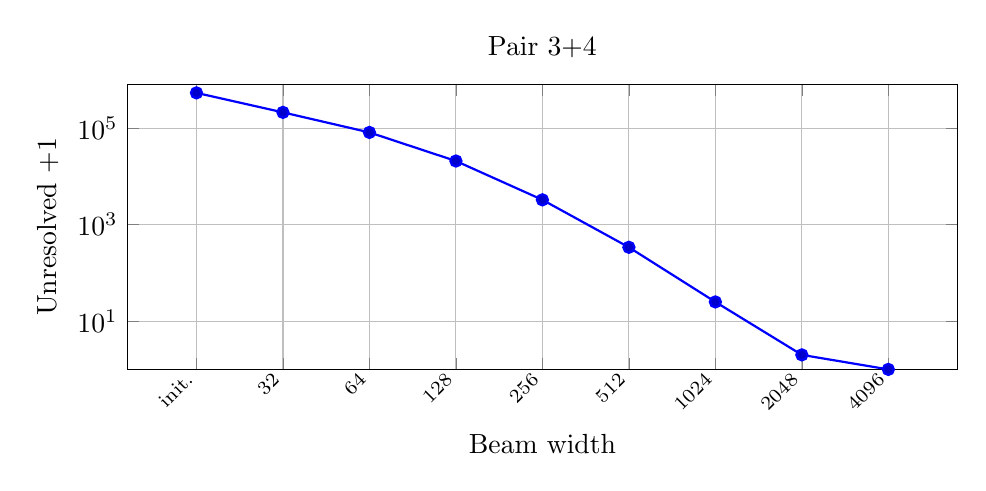
\begin{tikzpicture}
\begin{semilogyaxis}[
  width=\linewidth,height=52mm,title={Pair 3+4},
  xlabel={Beam width},ylabel={Unresolved $+1$},
  xtick={0,1,2,3,4,5,6,7,8},
  xticklabels={init.,32,64,128,256,512,1024,2048,4096},
  x tick label style={rotate=45,anchor=east,font=\scriptsize},
  ymin=1,ymax=800000,grid=major
]
\addplot+[mark=*,thick] coordinates {
  (0,536370) (1,211558) (2,81276) (3,20786) (4,3260)
  (5,339) (6,25) (7,2) (8,1)
};
\end{semilogyaxis}
\end{tikzpicture}
\end{minipage}\hfill
\begin{minipage}{0.49\linewidth}
\centering
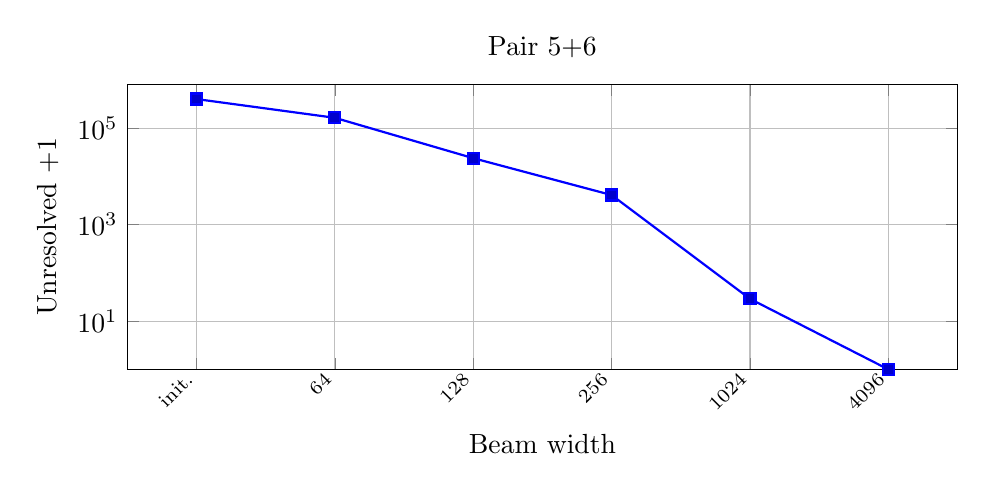
\begin{tikzpicture}
\begin{semilogyaxis}[
  width=\linewidth,height=52mm,title={Pair 5+6},
  xlabel={Beam width},ylabel={Unresolved $+1$},
  xtick={0,1,2,3,4,5},
  xticklabels={init.,64,128,256,1024,4096},
  x tick label style={rotate=45,anchor=east,font=\scriptsize},
  ymin=1,ymax=800000,grid=major
]
\addplot+[mark=square*,thick] coordinates {
  (0,399168) (1,163328) (2,23784) (3,4095) (4,29) (5,1)
};
\end{semilogyaxis}
\end{tikzpicture}
\end{minipage}
\caption{Unresolved direct-certificate obligations after each executed tier,
plotted as count plus one so that completion is represented exactly at one.
The pair-3+4 checkpoint changes within width 32; pair 5+6 changes checkpoint
between widths 64 and 128.}
\label{fig:survivor-curves}
\end{figure}

On an NVIDIA A100 80GB PCIe GPU with bfloat16 inference, active model-search
time was approximately 2~h 21~min 42~s for pair 3+4 and 3~h 53~min 44~s for
pair 5+6, or about 6~h 15~min in total.  These totals exclude phase-table
construction, exact rewriting, process gaps, and final replay.  Training logs
through the certificate-generation checkpoints record approximately 4.6
GPU-hours in total.  The point is not that every certificate had equal cost:
survivors required wider tiers in this run, and those widths were applied to
progressively smaller populations.

\begin{table}[t]
\centering
\caption{Lengths of direct neural-guided certificates.  Exact-rewrite words
are excluded.}
\label{tab:direct-word-lengths}
\small
\begin{tabular}{@{}lrrrrr@{}}
\toprule
Pair & Minimum & Median & Mean & Maximum & At maximum\\
\midrule
3+4 & 14 & 20 & 19.78 & 21 & 172,838\\
5+6 & 14 & 23 & 22.60 & 25 & 65,139\\
\bottomrule
\end{tabular}
\end{table}
These are lengths of words found by the portfolio, not shortest-distance
measurements or lower-bound witnesses.  The complete histograms appear in
\cref{app:word-lengths}.

\subsection{What the cascade data do and do not establish}

The published execution achieves complete coverage, but it is not a controlled
ablation.  Later tiers operate on distributions selected by earlier tiers, and
both pairs change checkpoint during the schedule.  Pair 3+4 also combines a
partial epoch-1024 pass with the epoch-1120 pass at width 32, while pair 5+6
changes from epoch 864 to epoch 3744 after width 64.  Consequently the rows do
not identify a pure width effect, and throughput measurements from different
tiers are not directly comparable.

We therefore make a narrower empirical claim: this particular portfolio found
bounded, independently replayable words for all 935,536 states left after exact
rewriting, within the reported hardware budget.  Establishing superiority to
IDA*, A*, a single fixed-width beam, or another learned policy would require a
separate controlled benchmark.  The certified upper bounds do not depend on
the outcome of such a comparison.

\subsection{Limitations}

The method is tailored to a one-move improvement, where only the product of
two maximal layers needs special treatment.  Larger reductions would generally
require certifying thicker boundary bands or a stronger structural argument.
The current neural targets are noisy random-walk depths, not exact distances;
the models have no admissibility guarantee.  Finally, the local bounds are
unconditional only for the two subgroup transitions reconstructed here.  The
112- and 111-move statements inherit the external assumptions made explicit in
\cref{cor:conditional-112,cor:conditional-111}.

\section{Artifact and reproducibility}
\label{sec:reproducibility}

The complete artifact is available at
\url{https://github.com/AnanasClassic/megaminx_34_56_phases_reduction}
\cite{kuznetsov2026artifact}.
It contains the paper sources, compressed SQLite certificate databases, both
certificate-generation checkpoints for each pair, training and cascade logs, pinned
problem manifests, independent verifier source, and scripts for reconstructing
all omitted intermediate tables.  The bibliography pins the exact artifact
commit used for this manuscript; the repository landing-page URL is provided
only for navigation.  No DOI or third-party archival deposit is claimed at the
time of writing.

The artifact supports three levels of reproduction:
\begin{enumerate}
  \item \textbf{Package audit.}  \texttt{make verify-package} streams both
    compressed databases, verifies compressed and uncompressed hashes, checks
    their schemas and complete distributions, and verifies all checkpoint
    hashes.  It does not require a neural framework or regenerated tables.
  \item \textbf{Proof reproduction.}  \texttt{make verify-pair34} and
    \texttt{make verify-pair56} fetch the digest-pinned source snapshot,
    recompute the subgroup orders from the committed action manifests, rebuild
    the table generator and replay implementations, regenerate the phase
    tables, maximal records, physical products, equivalence analysis, and exact
    rewrites, and replay every certificate.  The neural checkpoints are not
    loaded.
  \item \textbf{Discovery reproduction.}  The pair-specific training and
    cascade scripts retrain a model or rerun certificate discovery on a GPU.
    Because neural training and parallel floating-point execution need not be
    bit-reproducible, success is judged only by the same deterministic
    certificate checker.
\end{enumerate}

The proof environment requires Python~3.10 or newer, SymPy for the exact
Schreier--Sims audit, and the digest-pinned Go~1.22.3 container image.  The
published discovery run used an NVIDIA A100 80GB PCIe GPU with CUDA/bfloat16
inference.  Proof replay is CPU-only.  The historical problem-manifest builder
also accepts a p900 generator file with a pinned SHA-256 digest; that file is
not redistributed here.  It is construction provenance rather than a
proof-time dependency: the committed manifests are checked directly against
the physical move implementation and their group orders are recomputed.

The two compressed databases contain 536,369 and 399,167 direct records.  The
committed reference reports are historical Python-only outputs whose schemas
contain no Go transcript fields.  A full current reproduction emits a new
report containing the Go binary digest and the exact cross-language transcript
digest.  The repository also documents the 108-byte
physical state format, strict FTM word grammar, coordinate conventions,
artifact binary formats, and an explicit corruption-oriented threat model.
Code and computational data are distributed under the repository's stated
CC~BY-NC~4.0 terms, matching the license of the source dataset on which the
coordinate reimplementation is based.

\section{Conclusion}
\label{sec:conclusion}

The boundary-layer lemma turns two enormous combined subgroup-transition
questions into 944,200 concrete physical obligations.  Exact rewriting and
neural-guided beam cascades then provide a bounded word for every obligation,
while deterministic
coverage and replay keep all learned components outside the proof base.  The
result is the unconditional pair of ambient-FTM upper bounds
$\Rsolve_{\Omega}(G_5,G_7)\leq21$ and
$\Rsolve_{\Omega}(G_7,G_9)\leq25$, and the conditional
global arithmetic 112---or 111 when combined with the separate color-neutral
first-phase reduction.

The broader lesson is methodological.  Learned search can participate in an
exhaustive computational proof without itself being complete, interpretable,
or numerically trusted, provided that its output is a collection of small
classical certificates, a deterministic checker proves exact coverage, and
deterministic quotient and physical-state replay validates every direct word.
The full-reproduction workflow additionally requires a separately implemented
Go replay of the same transcript.  In the published run, the survivor cascade concentrated the widest
searches on the final 29 roots of a $935{,}536$-root direct obligation set.
Determining its advantage over fixed-width or non-neural alternatives requires
a controlled comparison.  A natural next step is to study when
the same boundary-layer construction extends to thicker bands and whether
controlled cascade policies can predict the appropriate search budget before
running the full certificate pass.


\appendix
\section{Published beam-cascade provenance}
\label{app:cascade}

\Cref{tab:pair34-cascade-full,tab:pair56-cascade-full} give the complete
per-tier provenance retained for the certificate-generation run.  Search time excludes
startup, validation, database-only skips, pauses, and independent replay.

\begin{table}[!ht]
\centering
\caption{Pair 3+4 cascade on an NVIDIA A100 80GB PCIe GPU.}
\label{tab:pair34-cascade-full}
\small
\begin{tabular}{@{}rrrrr@{}}
\toprule
Beam & Before & Newly certified & Remaining & Active time \\
\midrule
32   & 536,369 & 324,812 & 211,557 & 1:28:13$^{*}$ \\
64   & 211,557 & 130,282 & 81,275  & 0:25:44 \\
128  & 81,275  & 60,490  & 20,785  & 0:15:21 \\
256  & 20,785  & 17,526  & 3,259   & 0:08:28 \\
512  & 3,259   & 2,921   & 338     & 0:02:52 \\
1024 & 338     & 314     & 24      & 0:00:46.9 \\
2048 & 24      & 23      & 1       & 0:00:16.2 \\
4096 & 1       & 1       & 0       & 0:00:00.6 \\
\bottomrule
\end{tabular}
\par\smallskip
\footnotesize $^{*}$Combined epoch-1024 partial pass and epoch-1120 pass;
the first interval is reconstructed from certificate timestamps.
\end{table}

\begin{table}[h]
\centering
\caption{Pair 5+6 cascade on an NVIDIA A100 80GB PCIe GPU.}
\label{tab:pair56-cascade-full}
\small
\begin{tabular}{@{}rrrrr@{}}
\toprule
Beam & Before & Newly certified & Remaining & Active time \\
\midrule
64   & 399,167 & 235,840 & 163,327 & 2:55:41$^{*}$ \\
128  & 163,327 & 139,544 & 23,783  & 0:40:29 \\
256  & 23,783  & 19,689  & 4,094   & 0:10:44$^{\dagger}$ \\
1024 & 4,094   & 4,066   & 28      & 0:06:37 \\
4096 & 28      & 28      & 0       & 0:00:13.3 \\
\bottomrule
\end{tabular}
\par\smallskip
\footnotesize $^{*}$Reconstructed from timestamps for the older low-batch
implementation.  $^{\dagger}$Combined across an interrupted and resumed tier.
\end{table}

\section{Direct-certificate length distributions}
\label{app:word-lengths}

\begin{table}[!ht]
\centering
\caption{Exact histograms queried from the two direct-certificate databases.
The exact-rewrite partition is not included.}
\label{tab:direct-length-histograms}
\small
\begin{tabular}{@{}rrr@{\qquad}rrr@{}}
\toprule
Length & Pair 3+4 & Pair 5+6 & Length & Pair 3+4 & Pair 5+6\\
\midrule
14 & 8 & 1      & 20 & 168,765 & 32,170\\
15 & 245 & 17   & 21 & 172,838 & 54,632\\
16 & 2,631 & 122 & 22 & -- & 72,735\\
17 & 16,279 & 942 & 23 & -- & 79,404\\
18 & 56,097 & 4,392 & 24 & -- & 75,502\\
19 & 119,506 & 14,111 & 25 & -- & 65,139\\
\bottomrule
\end{tabular}
\end{table}

\section{Artifact entry points}
\label{app:commands}

The following commands are the intended top-level interfaces:
\begin{lstlisting}
make verify-package       # fast archive, schema, and checksum audit
make audit-tree           # reject caches and unintended publication files
make test                 # unit and corruption-oriented tests
make verify-pair34        # regenerate and certify phases 3+4
make verify-pair56        # regenerate and certify phases 5+6
make paper                # build this manuscript and check its LaTeX log
\end{lstlisting}
The two complete reproductions may also be invoked together with
\texttt{make verify-all}.  Pair-specific scripts expose training and discovery
separately so that no GPU dependency is introduced into certificate replay.

\clearpage
\section{Fail-closed verification checklist}
\label{app:threats}

\begin{table}[!ht]
\centering
\caption{Selected failure modes and the corresponding checks.}
\label{tab:threat-checks}
\small
\renewcommand{\arraystretch}{1.12}
\begin{tabularx}{\textwidth}{@{}
  >{\raggedright\arraybackslash}p{0.34\textwidth}
  >{\raggedright\arraybackslash}X@{}}
\toprule
Failure mode & Required check \\
\midrule
Published counts truncate generation & Derive reachability and maximal layers
from regenerated tables; compare controls only afterward. \\
Two quotient integers are treated as a physical product & Construct a full
state and round-trip both phase coordinates and the intermediate state. \\
Wrong multiplication or replay direction & Check the physical lifting
identities and replay every stored optimal word left-to-right. \\
Duplicate elimination hides a raw pair & Store a raw-to-unique map and require
coverage for every raw ID, irrespective of injectivity. \\
Search database is partial or stale & Require the exact remaining-ID set and
metadata hashes of the state, problem, and reduction artifacts. \\
Malformed or over-length move word & Use a strict canonical parser, count FTM
tokens, and enforce the pair-specific limit before replay. \\
Shared transition bug accepts a false word & Replay in the combined quotient,
the separately implemented Python physical model, and the Go physical verifier. \\
Neural score is mistaken for proof & Never load a checkpoint during proof
reproduction; accept only replayed words. \\
\bottomrule
\end{tabularx}
\end{table}


\begingroup
\small
\bibliographystyle{abbrv}
\bibliography{references}
\endgroup

\end{document}
